\section{Galaxy Selection and Size Measurement}
\label{sec:sample_methods}

In this section we describe our galaxy sample, and describe the two measurement methods used to derive sizes. 

\subsection{Extracting the galaxy sample}
\label{sec:sample}

To ensure all galaxies in the sample have enough particles to be considered morphologically resolved, we omit all subgroups with fewer than 100 stellar particles ($N_\star<100$). We apply a 95 per cent completeness criterion, dividing the sample of galaxies into those above and below the completeness limits in mass and luminosity. These completeness limits are given by the mass and luminosity at which the galaxy sample is missing 5 per cent due to galaxies having $N_\star<100$. We adopt 95 per cent complete rather than 100 percent complete to avoid the luminosity threshold being defined by anomalously bright galaxies with $N_\star<100$. These limits are presented in \tab{complete} at each redshift for the far UV band. This ensures we present results motivated by a complete galaxy sample. We nonetheless present the incomplete sample at low opacity in all scatter plots for context.

\begin{table*}
\begin{center}
\begin{tabular}{ c | c | c | c }
 \hline
 Redshift ($z$) & $\log_{10}(M/M_\odot)$ & $\log_{10}(L_{\mathrm{int}}/[\mathrm{erg} / \mathrm{s} / \mathrm{Hz}])$ & $\log_{10}(L_{\mathrm{att}}/[\mathrm{erg} / \mathrm{s} / \mathrm{Hz}])$ \\ \hline
 12 & 8.16 & 28.60 & 28.43 \\  
 11 & 8.15 & 28.55 & 28.42 \\  
 10 & 8.15 & 28.52 & 28.39 \\  
 9 & 8.14 & 28.46 & 28.34 \\  
 8 & 8.13 & 28.40 & 28.28 \\  
 7 & 8.13 & 28.31 & 28.19 \\  
 6 & 8.12 & 28.24 & 28.12 \\  
 5 & 8.11 & 28.16 & 28.03 \\
 \hline
\end{tabular}
\caption{The mass and luminosity 95 per cent completeness limits for the galaxy sample in each redshift bin. The mass limits are consistent across all bands, but the luminosity limits are band specific. Here we present the far-UV (FUV, 1500 \AA) limits focused on for the majority of the analysis presented in this article.}
\label{tab:complete}
\end{center}
\end{table*}

We further distinguish between 2 morphological populations by applying a threshold derived from the intrinsic size-luminosity relation of $S \geq 10^{29}$ erg s$^{-1}$ Hz$^{-1}$ pkpc$^{-2}$ to their central surface flux density (i.e. the surface flux density within the half light radius). This threshold splits the sample into a population of centrally compact galaxies and a population of diffuse galaxies; in subsequent plots we will denote the compact population by coloured hexbins and the diffuse population by greyscale hexbins.

\begin{figure}
	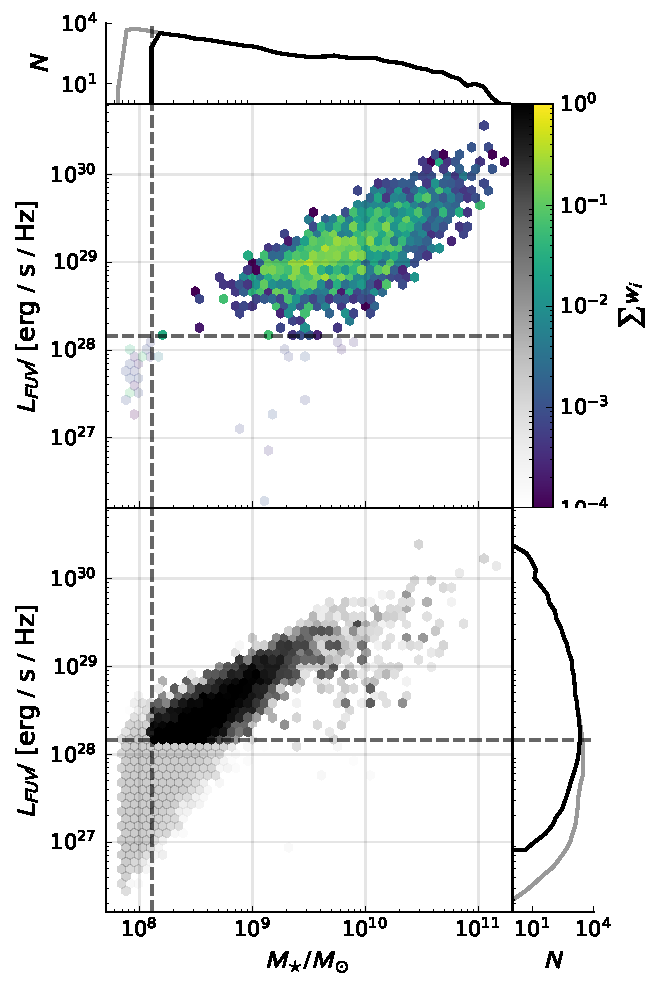
\includegraphics[width=\columnwidth]{Figures/MassLumin_FAKE.TH.FUV_5.0_sim_Intrinsic_default.pdf}
    \caption{The intrinsic mass-luminosity relation at $z=5.0$. The top panel of coloured hexbins are the galaxies in the compact population and the lower panel of greyscale points represent galaxies in the diffuse population, as described in \sec{sample}. The dashed lines show the completeness limits for the galaxy sample with those galaxies that fall outside this completeness threshold denoted by low opacity. Each hexbin is coloured by the weighted number density of galaxies, using the \flares\ region weighting scheme. The histograms on each axis show the total distribution of galaxies in both the compact and diffuse population along each axis, with the grey line showing all galaxies and the black line showing those with $N_\star\geq100$.}
    \label{fig:int_lumin_mass}
\end{figure}

This division of the galaxy sample is shown in the mass-luminosity relation in \fig{int_lumin_mass} at $z=5$; here we have adopted the previously described colouring and have used opacity to distinguish the complete and incomplete populations. The dashed lines denote the completeness limits in mass and luminosity. The histograms on the axes show the galaxy distribution along each axis with the full galaxy population in grey and galaxies with $N_\star\geq100$ shown in black. 

All following plots will follow these plotting conventions, with greyscale colours denoting the diffuse galaxy distribution and coloured hexbins denoting the compact population (as defined by their central surface density). The hexbins themselves indicate the weighted number density of galaxies, using the weights derived in \cite{Lovell2021}. All fits are performed on the complete sample. This division of the galaxy sample leads to:
\begin{itemize}
    \item 50238 galaxies in the sample with more than 100 stellar particles (25556, 2863 and 492 at $z=5$, $z=8$ and $z=10$ respectively).
    \item 7172 in the compact population with more than 100 stellar particles (2701, 696 and 240 at $z=5$, $z=8$ and $z=10$ respectively).
    \item 43066 in the diffuse population with more than 100 stellar particles (22855, 2167 and 252 at $z=5$, $z=8$ and $z=10$ respectively).
    \item 31697 galaxies in total above the completeness limit (16238, 1700 and 273 at $z=5$, $z=8$ and $z=10$ respectively).
\end{itemize} 


% \subsubsection{Detecting the diffuse galaxy sample}

% A further motivation for these cuts is the difficulty in reconciling the diffuse galaxy population with observations. At these high redshifts, differences in galaxy detection methods between observations and halo finders become more distinct with observational methods such as segmentation likely to break diffuse clumpy objects into smaller objects or miss the fainter structure linking them in the halo finder, especially at the survey depths possible at these redshifts. 

% This highlights the importance of treating synthetic observations as closely to true observations as possible to yield robust comparisons; particularly the importance of employing a treatment independent of the halo finder. We defer an analysis of this kind to a future paper investigating the differences in approach in the context of \flares. In this paper we instead focus on the complete (and mostly compact and bright) galaxy sample as detected by the halo finder and independent of observatory, including the diffuse and incomplete sample for context. 

\subsection{Size measurement methods}
\label{sec:measure}

There are a myriad of methods used to define the sizes of galaxies present in the literature including S\'ersic profile fitting \citep{Sersic1963, Sersic1968}, curves of growth \citep[e.g.][]{Ferguson_2004, Bouwens_2004, Oesch_2010}, Petrosian radius \citep{Petrosian1976},
and simulation specific methods, that use the particle distribution to find the radius enclosing a percentage of the total mass/luminosity. 

Each measurement method introduces its own dependencies and challenges. In this section we detail and compare the two methods utilised in this analysis: a particle based method, and a non-parametric pixel based method \citep[e.g.][]{Ribeiro2016, Ma_18_size, Marshall21}. We neglect curves of growth, Petrosian radius and S\'ersic profiles entirely; at these redshifts the clumpy nature of galaxies, particularly at lower masses \citep{Jiang_2013, Bowler2016}, make these methods unreliable. Throughout this work we use $R$ to refer to the half light radius (size) of a galaxy.

\subsubsection{Particle based method}

We take the underlying particle distribution within a 30 pkpc aperture and find the radius of the particle bounding half the total luminosity inside this aperture. We then interpolate around this initial measurement to better sample the radial density profile, mitigating it's discretisation into individual, comparatively low resolution, particles. 

It should be noted that this measurement method is sensitive to the chosen galactic centre; in this work we use the centre of potential calculated by SUBFIND. Other choices, such as the centroid, can give different results for diffuse and irregular structures since the centre of potential may be located within one of the clumps, which may not necessarily lie in the centre of the galaxy. This offset centre leads to larger size measurements, as the majority of the stellar material of the galaxy is offset from the centre from which the radius is measured.

In all plots including this measurement we take the luminosity to be the sum of each individual particle's luminosity within the aperture, neglecting any smoothing over the SPH kernel. 

% \subsubsection{Aperture based method}

% The aperture method (or the curve of growth method) applies 100 circular apertures with radii from 0.1 per cent the pixel size (the softening length) to $1/4$ of the total FOV of the image. This is guaranteed to enclose the half light radius of the galaxy while minimising the the number of apertures that need to be calculated, thus reducing the overall computation time. These apertures are then applied to the image and the resulting curve of growth is linearly interpolated to increase the aperture resolution to 10000 from 100 and minimise error. The interpolated aperture radius nearest to half the total luminosity of the image is then taken as the half light radius. This interpolation results in a maximum possible uncertainty in the half light radius measurement of 1.5 ppc. 

% [curve of growth plot?]

\subsubsection{Pixel based method}
\label{sec:pixel}

In the non-parametric pixel approach, the pixels of the image are ordered from most luminous to least luminous. We then find the pixel area containing half the total luminosity before converting to a radius assuming a circular area, $R=\sqrt{A/\pi}$, and then interpolating around this radius as in the particle method. Unlike the particle method this method of measurement has a minimum possible size where half the total luminosity falls within a single pixel, resulting in a radius of $R_{\mathrm{min}}=\sqrt{A_{\mathrm{pix}}/\pi}$ before interpolation between 0 and $R_{\mathrm{min}}$. The interpolation here allows for the measurement of half light radii smaller than a single pixel, however this does not remove the limitation caused by the finite pixel resolution.

This method is particularly robust at high redshifts, where the independence from a centre definition and non-contiguous size definition better encapsulate the morphology of clumpy structures.

In all plots using this measurement we present the luminosities as detected from the image, i.e. the sum of all pixels within the FOV. This can subtly differ from the particle luminosities where a particle's kernel extends beyond the bounds of the FOV, spreading the particles light outside the image in contrast to the particle based method.

\subsubsection{Comparing particle and pixel methods}

\begin{figure}
	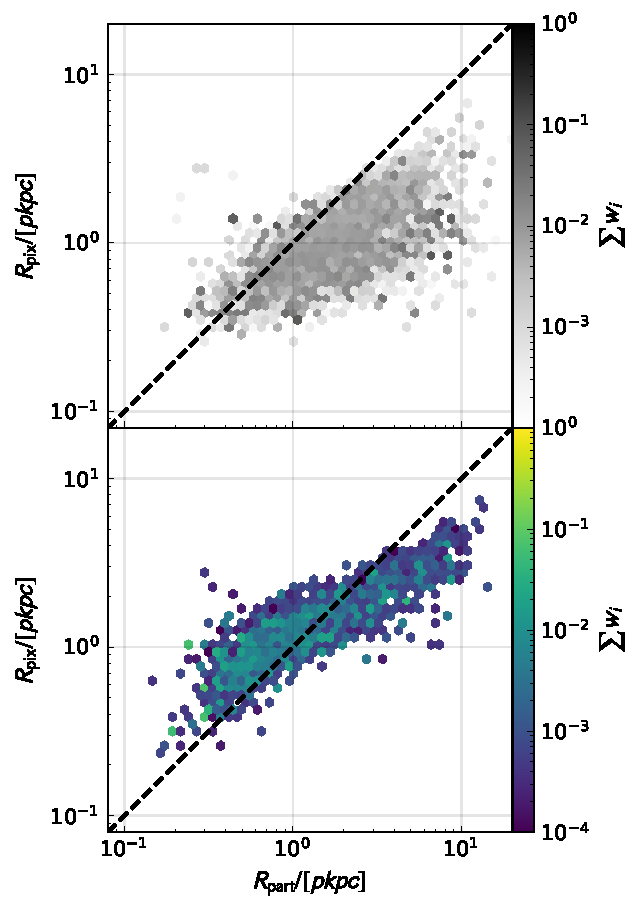
\includegraphics[width=\columnwidth]{Figures/ComparisonHalfLightRadius_FAKE.TH.FUV_5.0_sim_Total_default.pdf}
    \caption{A comparison between the dust attenuated half light radii of galaxies at $z=5$ yielded by the particle measurement method (x-axis) and the pixel method (y-axis). The upper panel of greyscale points show the diffuse galaxy population while the lower panel of coloured points show the compact galaxy population. The dashed black line corresponds to a 1:1 relationship. Each hexbin is coloured by the weighted number density of galaxies, using the \flares\ region weighting scheme.}
    \label{fig:size_method_comp}
\end{figure}

In \fig{size_method_comp} we present a comparison of these methods for the sizes of all galaxies at $z=5$ using their intrinsic luminosities. For the compact galaxies (colour) we see a reasonable correspondence between the two methods with a scatter around the 1:1 relation. However, as the size of a galaxy increases the particle method begins to produce larger sizes than the pixel method due to a combination of centring effects and luminous structures within the outskirts of galaxies, such as those shown in a number of panels in \fig{example_img}. Conversely, for the smallest galaxies, the pixel size is larger than the particle size; this is a manifestation of the stellar particle smoothing used in the creation of the images, where light concentrated in densely packed particles is smoothed over a larger pixel area. 

For the diffuse (greyscale) population the scatter is more pronounced and extends towards larger particle values across the full range of sizes. This is because of the aforementioned strength of the pixel method when it comes to clumpy diffuse structures and the issue of defining a centre for these structures in the particle method. The size floor is also evident in the smallest galaxies in the diffuse (and incomplete) sample where a single pixel contains half the total luminosity of the dim galaxy. 

\section{Size-Luminosity relations}
\label{sec:size-lumin}

% Add here a summary of what will be shown in this section, short and sweet. (LOS gradient + dust gradient)
% Summary of papers that we have compared to
% Introduce subsections

Here we present results for the sizes of galaxies in the epoch of reionisation. All plots that compare to observational quantities are derived from the pixel measurement method (\sec{pixel}) measured from the synthetic images detailed in \sec{image}. Intrinsic properties such as the intrinsic size-luminosity relation (\sec{intrinsic}) and half dust radius (\sec{dustdist}) are measured using the particle method to focus on the intrinsic nature of these properties.

\subsection{Intrinsic UV size-luminosity relation}
\label{sec:intrinsic}

\begin{figure}
	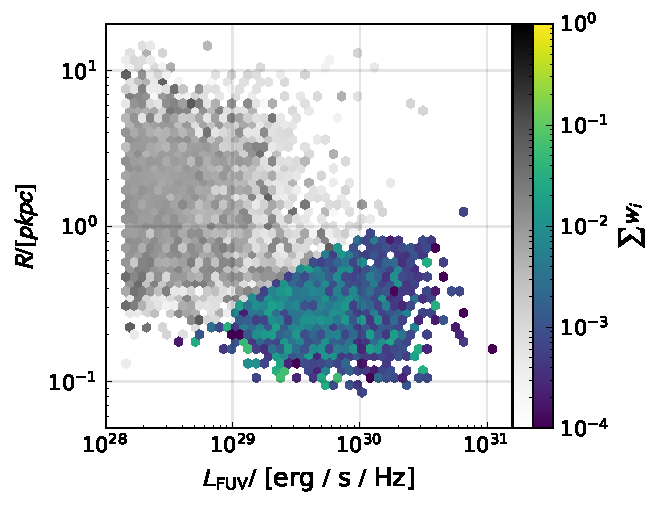
\includegraphics[width=\linewidth]{Figures/HalfLightRadius_part_FAKE.TH.FUV_5.0_sim_Intrinsic_default.pdf}
    \caption{The intrinsic UV size-luminosity relation at $z=5.0$, measured using the particle method. Showing the dimmer diffuse population in greyscale and the bright compact population in colour. The hexbins are coloured by the sum of \flares\ region weightings for each individual galaxy, making each hexbin a weighted number density in the UV size-luminosity plane.}
    \label{fig:int_hlr}
\end{figure}

\begin{figure*}
	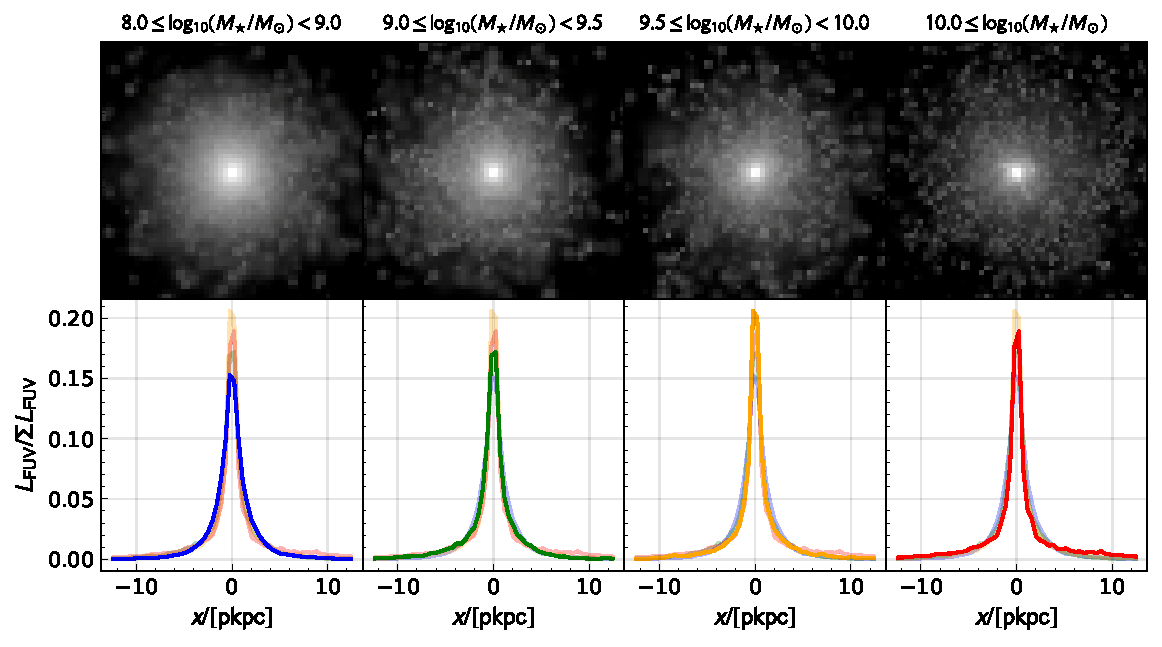
\includegraphics[width=\linewidth]{Figures/StackLogImgRow_FAKE.TH.FUV_00_010_z005p000_sim_Intrinsic_default.pdf}
    \caption{The upper panel contains stacked individually log-scaled images of the intrinsic luminosity of every galaxy in our complete galaxy sample at $z=5$. These stacks cover the central $\sim24$ pkpc of the image and are split into mass bins (increasing left to right). The lower panels show 1-dimensional profiles of these stacks. The luminosity on the y-axis of these profiles is normalised to the sum of each stacked image. In each panel all profiles are plotted with the curves corresponding to the other panels plotted in low opacity to aid interpretation.}
    \label{fig:int_stack}
\end{figure*}

Although not probed in observations, we can use the intrinsic UV size-luminosity relation to trace the underlying stellar population in galaxies. \fig{int_hlr} shows this relation at $z=5$ for the particle measurements. This shows two surprising features: 2 distinct populations, and a clear negative slope to the intrinsic size-luminosity relation. 

Although the negative slope of the intrinsic size-luminosity relation is somewhat counter intuitive, it has been seen at these redshifts in other recent simulations, particularly in \bluetides\ \citep{Marshall21} with a negative size-mass relation at $z=7$ and \textsc{Illutris-TNG} \citep{Popping2021} with a negative observed-frame 850 $\mu$m size-mass relation at $z=5$. Indeed, there are also hints in observations with evidence for a constant dependence between galaxy size and mass \citep{Lang_2014, Mosleh_2020}. 

Here the division in central surface density is particularly evident. In terms of luminosity we have one dim ($L\lesssim10^{29}$ erg s$^{-1}$ Hz$^{-1}$) and more diffuse population, and one bright ($L\gtrsim10^{29}$ erg s$^{-1}$ Hz$^{-1}$) and compact ($R_{1/2}\lesssim 1$ pkpc) population.

We will present our investigation into the physical mechanisms governing this bi-modality in detail in an upcoming paper, but for context in \flares\ (the \eagle\ model):
\begin{itemize}
    \item At $z\gtrsim5$, galaxies that reach $M/\mathrm{ M}_\odot\gtrsim10^9$ develop extremely dense cores and begin a spike in core star formation at high stellar birth densities.
    \item This begins to seed the gas in the galaxy's core with metals, increasing the effectiveness of metal line cooling, inhibiting stellar and AGN feedback, and further driving star formation. 
    \item This overcooling causes a feedback loop of star formation in the galaxy's core, allowing the galaxy to become massive and ultra compact during this early epoch. 
    \item While this process takes place in the galaxy's core the galaxy accretes an extended gas distribution up to 100 times larger than the stellar distribution. Due to the high densities in the core, stellar feedback is unable to mix the core's metals into this surrounding gas distribution. This lack of metals inhibits cooling and leaves the extended gas distribution unable to efficiently form stars.
    \item At $z\lesssim4$ the extended gas distribution reaches the density and metallicity necessary for efficient star formation. This is facilitated partly by their own collapse and partly due to the growing efficiency of stellar and AGN feedback \citep{crain_eagle_2015}, mixing metals from the core into the surroundings. This extended star formation manifests as an increase in galaxy size at late times, yielding the size distribution we see at the present day.
\end{itemize}

In the upper panel of \fig{int_stack} we present a stack of the central intrinsic emission of all galaxies at $z=5$ in \flares\ (irrespective of completeness) split into mass bins of $\log_{10}(M/M_\odot)=[8-9, 9-9.5, 9.5-10, >10]$. This qualitatively shows how the negative gradient in the size-luminosity relation translates to the compactification of a galaxy's intrinsic emission in relation to a galaxy's mass. In the lower panel of \fig{int_stack} we plot 1-dimensional profiles of the stacked mass bin images to explicitly show the compactification. As with the stacked images, the profiles exhibit a narrowing and increasing central concentration with increasing mass. The overcooling begins to take effect between the left most mass bin ($10^{8}<M/M_\odot<10^{9}$) and the next mass bin of $10^{9}<M/M_\odot<10^{9.5}$. At this crossover between regimes there is a narrowing of the profile and stronger concentrated peak, which becomes more peaked as the mass increases. The growth of this central peak then drops off in the final mass bin due to an increased contribution by the wings of the profile; galaxies in this mass bin exist in the most dense environments and thus include more luminous substructure at large radii.

% These galaxies then continue their evolution accreting large non-star forming extended gas distributions which eventually begin star formation around $z\sim3-4$, driving the sizes of galaxies in this regime to sizes consistent with those observed at lower redshifts.

% This bi-modal distribution in size is seen at high redshift in many simulations with different subgrid prescriptions [REFS]. However, as plausible as this scenario sounds the question stands whether this behaviour is physical or numerical. We will investigate in \sec{dust} whether this scenario is compatible with observations after the inclusion of dust.

% In this paper we focus on the sizes as produced by the halo finder but it should be noted that this negative gradient is present in many simulations [REFS], however, the exact structure of this bi-modality is highly sensitive to not only the subgrid model of the simulation but also the halo finder techniques used for structure extraction and the methods use to make and detect the synthetic galaxy images. 

% The later of these sensitivities is clear when comparing \fig{int_hlr} to \fig{int_hlr_pix}. The pixel method for measurement displays a significantly decreased maximal size with a much shallower negative trend to the size luminosity distribution. This shows just how diffuse and clumpy the galaxies populating the upper left hand corner in \fig{int_hlr} are with the non-contiguous approach of the pixel method accounting for the clumpy nature of these diffuse galaxies to produce a maximal size $\approx1$ dex smaller than the underlying particle method distribution. We can also see a $\approx0.2$ dex increase in the minimal measured size for luminous compact population with the pixel method which is the single pixel limit of this method.


\subsection{The effects of dust}
\label{sec:dust}

We now move on from the intrinsic size-luminosity relation to discuss the effects of dust on the observed UV size-luminosity relation. All plots from this point on will present the pixel measured sizes unless explicitly stated otherwise.

\subsubsection{The distribution of dust}
\label{sec:dustdist}

\begin{figure}
	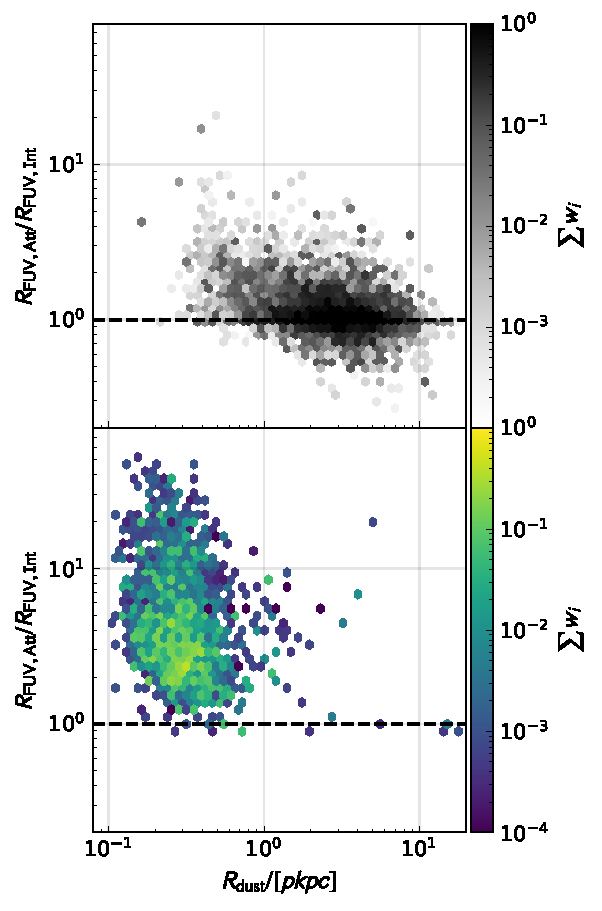
\includegraphics[width=\columnwidth]{Figures/HalfDustRadius_hlrratio_FAKE.TH.FUV_5.0_Intrinsic_sim_default.pdf}
    \caption{The ratio between dust attenuated and intrinsic size as a function of the half dust radius (the radius enclosing half the mass in gas-phase dust) for all galaxies at $z=5$, computed using the particle method. Once again, the galaxy sample is divided into the diffuse population (upper, greyscale) and the compact population (lower, coloured) and the hexbins are coloured by the cumulative weighting of each galaxy within a hexbin.}
    \label{fig:HDR}
\end{figure}

Dust attenuates the intrinsic stellar emission making observations of the pure stellar emission impossible. The affect this obfuscation will have on the measured size of a galaxy is sensitive to the spatial distribution of dust in a galaxy: a uniform screen would have no discernible effect on the size, whereas any concentration of dust in a particular region will have important consequences for the spatial distribution of observed stellar emission, and therefore perceived size. 

We probe the underlying dust distribution in these galaxies by calculating the half dust radius (i.e. the radius enclosing half the mass in gas-phase dust). To calculate the gas-phase dust mass we use the metallicity of each gas particle and multiply by the galaxy specific $\mathrm{DTM}$ (described in \sec{dustatt}) to get the dust mass of each gas particle. 

\fig{HDR} shows the ratio between attenuated and intrinsic particle based sizes as a function of this half dust radius at $z=5$. Galaxies in the compact population (coloured hexbins) have dust distributions with $R_{1/2, \mathrm{dust}} \lesssim 1$ pkpc and $R_{\mathrm{att}}/R_{\mathrm{int}}\gtrsim1$. This indicates that, in the compact galaxy sample, not only is the distribution of dust highly concentrated in the core of the galaxy, but the more concentrated the dust, the larger the increase in observed size due to the attenuation of the galaxy's bright core\footnote{This strong attenuation of the core justifies the omission of the AGN contribution to the UV luminosity. We have confirmed the AGN contribution is heavily attenuated at these wavelengths, in fact only a handful of galaxies in the sample have AGN that are comparable to their host galaxy in the UV luminosity.}. 
With the central regions strongly attenuated, the more extended regions are able to contribute more to the total luminosity of the galaxy, increasing the perceived size. In the most extreme cases, galaxies can appear $\sim50$ times larger when including dust attenuation.

The vast majority of the diffuse galaxy population (greyscale) also have diffuse dust distributions ($R_{1/2, \mathrm{dust}} > 1$ pkpc) and exhibit a more conservative increases in size between intrinsic and attenuated size. Compared to the compact population, the more diffuse dust distributions (and galaxies) have a flatter relation between the ratio of sizes and half dust radius. Both the smaller increase in size and the flattening of this relation can be explained by a more uniform distribution of dust in these diffuse clumpy structures\footnote{Those galaxies in the diffuse population that do not follow this trend (i.e. exhibit large increases in size with the inclusion of dust and have compact dust distributions) are galaxies very close to the central surface flux density threshold used to split the populations.}.

Galaxies that fall below the dashed line, indicating a ratio of 1, represent a decrease in size with the inclusion of dust effects. These are instances where the dust is more uniformly distributed, and results in greater attenuation of their extremities, driving down the apparent size.

\subsubsection{The Observed UV size-luminosity distribution}

\begin{figure*}
  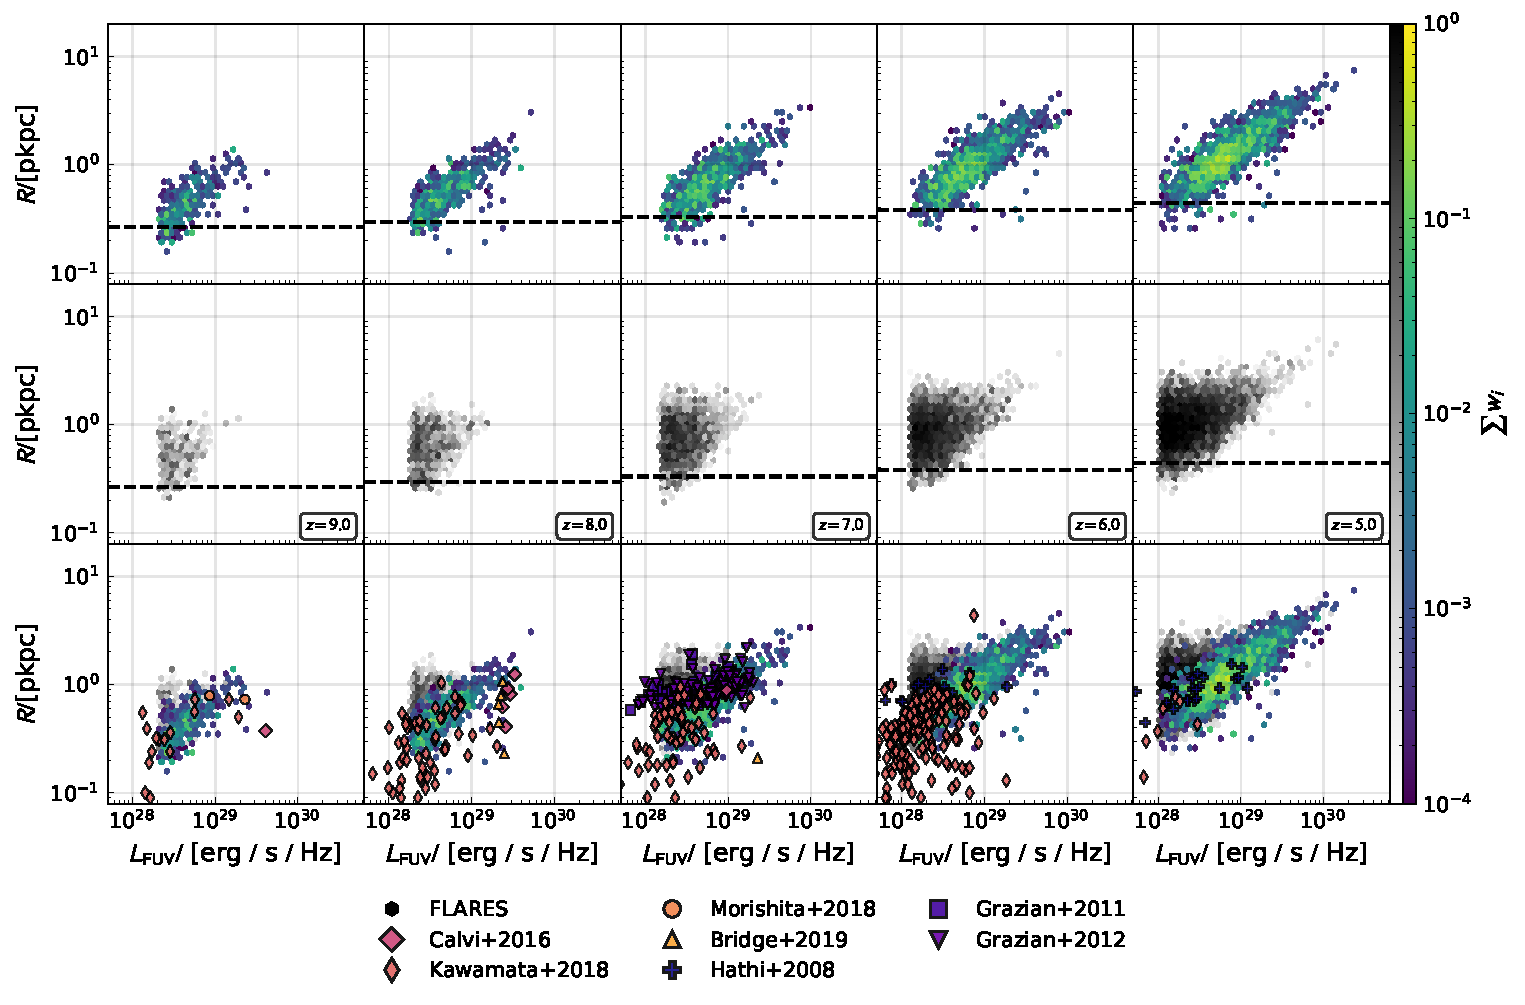
\includegraphics[width=\linewidth]{Figures/HalfLightRadius_pix_FAKE.TH.FUV_sim_Total_default.pdf}
  \caption{The attenuated far-UV (1500 \AA) size-luminosity relation measured using the pixel method. The hexbins are again coloured by the weighted number density. The galaxy sample is divided into the compact galaxy population (top row, colour) and the diffuse galaxy population (middle row, greyscale). The dashed line shows the pixel resolution of the images used to make the \flares\ measurements. Galaxies can fall below this line due to the interpolation used in the calculation of the pixel half light radius. The bottom row contains both galaxy populations with a comparison to high redshifts observations using the Hubble space telescope \citep{Hathi_2008, Grazian2011, Grazian_2012, Calvi_2016, Kawamata_2018, Morishita_2018, Bridge_2019}.}
  \label{fig:HLR_with_dust_obscomp}
\end{figure*}


The negative gradient in the intrinsic size-luminosity relation presented in \fig{int_hlr} is in direct conflict with observational results which necessarily include the effects of dust attenuation \citep[e.g.][]{Hathi_2008, Grazian2011, Grazian_2012, Shibuya2015, Calvi_2016, Kawamata_2015, Kawamata_2018, Morishita_2018, Bridge_2019, Bouwens2021, Yang2022}. However, in \sec{dustdist} we have shown that the inclusion of dust attenuation can result in large increases in size for the most intrinsically compact galaxies. Ascertaining if this effect is enough to yield sizes in line with observations is imperative to probe the validity of the negative intrinsic size-luminosity relation, and thus the physical models used in \flares. 

To compare to the observed results we use the method detailed in \sec{image} for synthetic image creation and the pixel measurement method (\sec{pixel}) to produce the observed size-luminosity relation and compare to a wide array of observations in integer redshift bins from $z=5-9$. This observed size-luminosity relation is shown in \fig{HLR_with_dust_obscomp}. 

Evidently, the concentration of dust in compact cores and increase in size between intrinsic and attenuated sizes, detailed in \sec{dustdist}, has completely reversed the slope of the size-luminosity relation relative to the intrinsic relation. 

Focusing on the high central surface density distribution (coloured hexbins), beyond the positive relation between size and luminosity, we can already see a power law relation with minimal scatter. This scatter is increased for the diffuse, low central surface density population (greyscale hexbins), particularly for low luminosity galaxies which exhibit a large range of sizes at fixed luminosity. We can also see that the \flares\ galaxy sample extends to larger sizes and higher luminosities than the observed results, this is because of \flares's focus on rare and extreme environments where the most luminous galaxies reside.

There is a fair agreement between the scatter of observational measurements and the \flares\ distribution with the exception of galaxies in the \cite{Kawamata_2018} (lensed) sample which have sizes smaller than the resolution of \flares. Particularly evident when comparing the \flares\ and observational scatter are the \cite{Grazian2011} and \cite{Hathi_2008} (dropout selected) points at $z=7$ and $z=6$, respectively, with similar normalisation to the low central surface density galaxies which scatter further from the power law relation evident in the compact population. This could be tantalising observational evidence for the galaxies that populate the diffuse population.

\begin{figure*}
  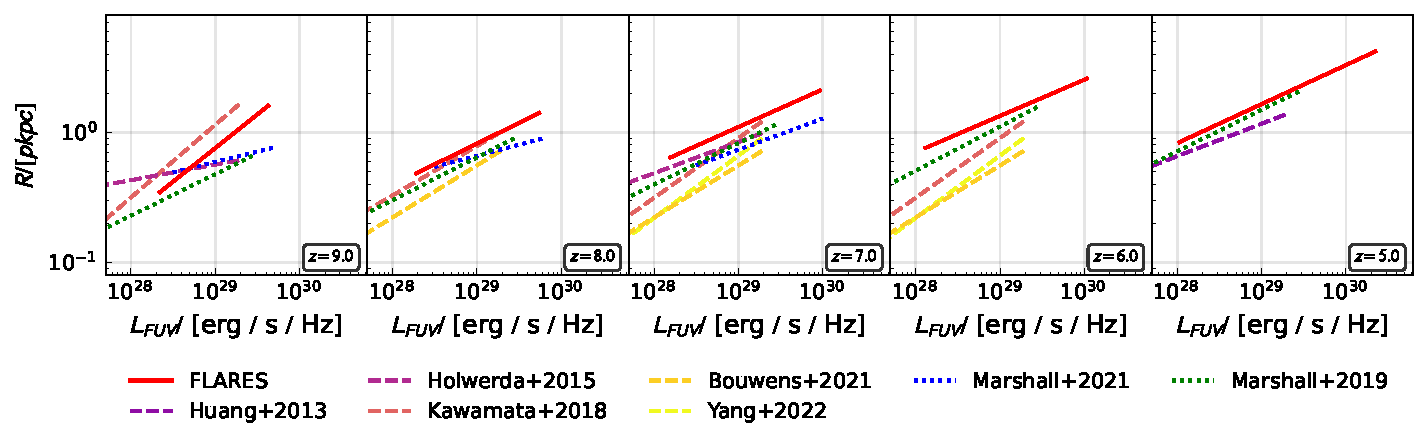
\includegraphics[width=\linewidth]{Figures/FitHalfLightRadius_pix_FAKE.TH.FUV_sim_Total_default_Complete.pdf}
  \caption{Fits to the UV size-luminosity relation including the effects of dust measured using the pixel method. To perform the fits we use the entire complete galaxy sample. We include comparisons to observations without lensed galaxies \citep{Huang_2013, Holwerda_2015}, observations including lensed sources \citep{Kawamata_2018, Bouwens2021, Yang2022} and simulations \citep{Marshall2019, Marshall21}. We denote \flares\ by a red solid line, observations by dashed lines and other simulations by dotted lines.}
  \label{fig:fits_obscomp}
\end{figure*}

\begin{table*}
\begin{center}
\begin{tabular}{ c | c | c | c }
 \hline
 Redshift ($z$) 
 & $R_0/ [\mathrm{pkpc}]$ & $\beta$ \\ \hline
 9 
 & 0.793$\pm$0.019 & 0.519$\pm$0.026 \\
 8 
 & 0.842$\pm$0.012 & 0.319$\pm$0.013 \\  
 7 
 & 1.126$\pm$0.011 & 0.290$\pm$0.008 \\
 6 
 & 1.370$\pm$0.007 & 0.279$\pm$0.004 \\
 5 
 & 1.692$\pm$0.006 & 0.300$\pm$0.003 \\
 \hline
\end{tabular}
\caption{The fitting results for \eq{size_lumin_fit} for each redshift bin in \fig{fits_obscomp} for the attenuated size-luminosity relations, measured using the pixel method (\sec{pixel}). $R_0$ is a normalisation factor, and $\beta$ is the slope of the size-luminosity relation.}
\label{tab:rfit}
\end{center}
\end{table*}

To quantify the agreement between the observational scatter and the \flares\ sample we use \texttt{curve\_fit} (non-linear least squares fitting), from \texttt{scipy} \citep{2020SciPy-NMeth}, to produce fits of the form of \eq{size_lumin_fit}. The results of this fitting are shown in \tab{rfit}.

\fig{fits_obscomp} shows a comparison of these fits (solid red lines) to fits from observed samples: \cite{Huang_2013} at $z=5$, \cite{Holwerda_2015} at $z=7$ and $z=9$, \cite{Kawamata_2018} at $z=6-9$, \cite{Bouwens2021} at $z=6-8$, and \cite{Yang2022} at $z=6-7$, the latter 3 of these including lensed sources. We also compare to two simulations: the \textsc{Meraxes} semi-analytic model \citep{Liu_meraxes, Marshall2019} at $z=5-9$, and the \bluetides\ simulation \citep{Marshall21} at $z=7-9$. We denote observations with dotted lines and simulations (other than \flares) by dotted lines. Each fit is plotted using their published fitting parameters.

At $z>7$ the \flares\ fits exhibit a good agreement in slope with the observational studies including lensed samples. These fits are significantly steeper than the observational samples that do not have a contribution of lensed galaxies, as demonstrated in \cite{Bouwens2021}. At $z\leq7$ the \flares\ fits begin to flatten relative to the studies including lensed sources as galaxies in the dim and diffuse size-luminosity regime become more numerous. 

Compared to \bluetides, we find \flares\ has a steeper size-luminosity relation at $z=8-9$ and a stronger redshift evolution in the normalisation over the redshift range $7\leq z \leq9$. With respect to \textsc{Meraxes} we find a good agreement in slopes at $z<9$ with a consistently higher normalisation at all redshifts.

Each work predicts a different normalisation of the size-luminosity relation. This is particularly evident at $z<8$ where \flares\ has consistently higher normalisation than all other studies. One explanation for this difference is the resolution and measurement methods in each study. The pixel method used in this work is sensitive to the resolution of the image (for which we adopt the softening length of the simulation), observational studies on the other hand use images with a higher resolution than the softening length of \flares\ and use an array of measurement techniques that are less sensitive to the pixel resolution. \bluetides\ uses the pixel method but adopts a higher pixel resolution below the softening length of the simulation and \textsc{Meraxes} derive their sizes (scale radius of the disc) from the SAM galaxy properties. In addition to methodological differences, there is likely a significant contribution to the normalisation by the diffuse galaxies, which at fixed luminosity extend to larger sizes in the \flares\ sample. 

The slopes reported in \tab{rfit} for the attenuated size-luminosity relation are in broad agreement with the results of \cite{Grazian_2012}, \cite{Huang_2013}, \cite{Holwerda_2015}, \cite{Shibuya2015}, \cite{Kawamata_2018}, \cite{Bouwens2021} and \cite{Yang2022} in various different redshift regimes. At $z>7$ the \flares\ results exhibit the steeper slopes present in \cite{Kawamata_2018}, \cite{Bouwens2021}, and \cite{Yang2022} before flattening into closer agreement with \cite{Grazian_2012}, \cite{Huang_2013}, \cite{Holwerda_2015} and \cite{Shibuya2015} at $z\leq7$. Again, this is due to the aforementioned compact low luminosity galaxies present in the lensed samples, which are absent from the other studies, and the diffuse low luminosity galaxies in the \flares\ sample which become more numerous with decreasing redshift. 

Many of the compact galaxies that strongly affect the slope of the size-luminosity relation in lensing studies fall below the resolution limit of \flares\ (indicated by the dashed line in \fig{HLR_with_dust_obscomp}) and \bluetides. Higher resolution simulations are necessary to ascertain if these galaxies are present in the simulated sample and produce the same steepening behaviour. All observational samples also lack the most diffuse galaxies in the simulated samples due to their low surface densities. These would act to flatten the size-luminosity relation if present. Future works will aim to address both these issues with higher resolution simulations and fully synthetic observations including survey limits, instrument noise, point spread functions and observational methods of structure detection; the former addressing the missing dim and compact galaxies in the simulated sample and the latter addressing the diffuse galaxies which are likely undetected in the observational sample.

\subsection{The size-luminosity relation as a function of wavelength}

\begin{figure*}
    \centering
	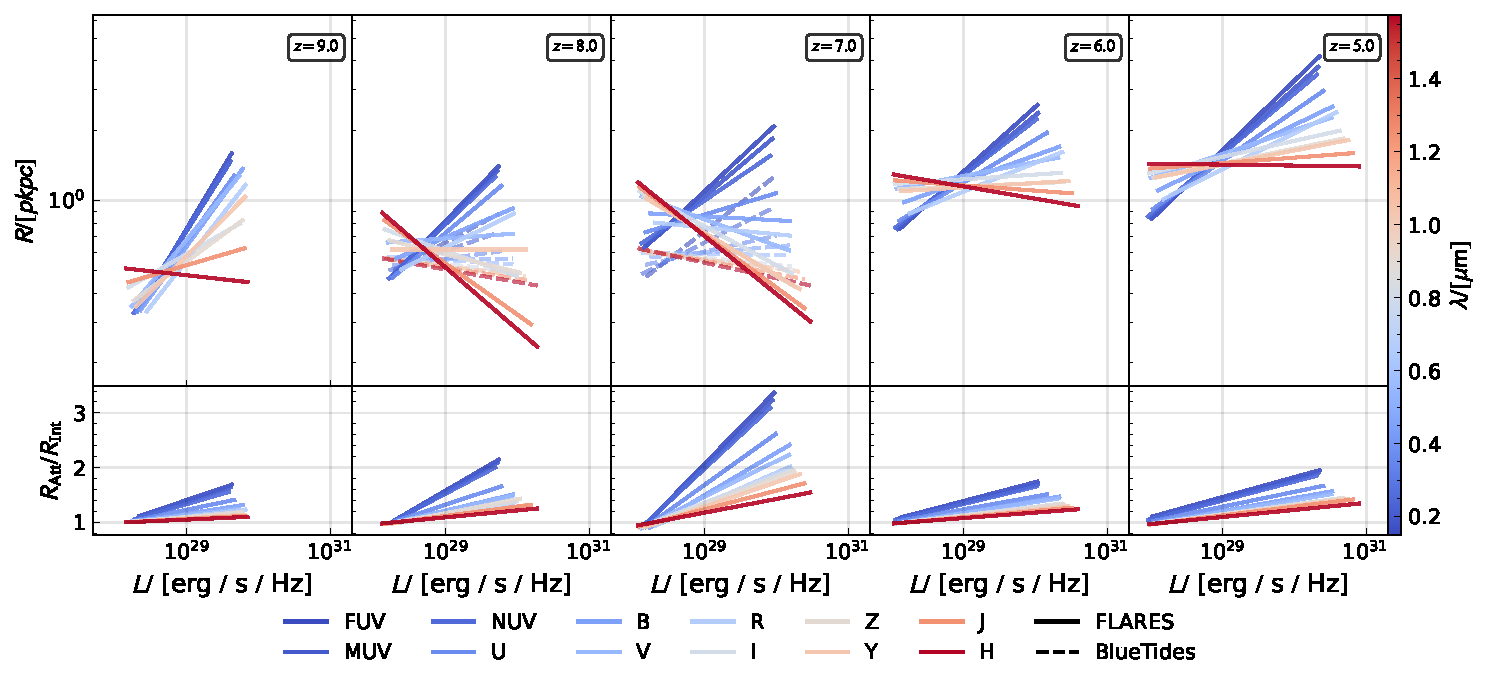
\includegraphics[width=\linewidth]{Figures/FilterCompHalfLightRadius_pix_Complete_sim_Total_default.pdf}
    \caption{The upper row of panels show fits to the size-luminosity relation for all rest frame bands in \fig{example_sed}. Solid lines represent the \flares\ fits while dashed lines show the \bluetides\ \citep{Marshall21} fits for the same selection of bands. The lower row of panels show straight line fits to the ratio between the intrinsic and attenuated sizes for each band. The colour of the line denotes the band, with the bluest bands in blue and reddest bands in red. The colorbar shows the central wavelength of each rest frame band in microns.}
    \label{fig:colors}
\end{figure*}

In \fig{colors} we present the size luminosity relation across a range of rest frame filters (shown in \fig{example_sed}), and compare to the corresponding fits from \cite{Marshall21} at $z=[8, 7]$. We present the fitting parameters in \app{bandtable}.

As the probed wavelength regime reddens, the slope of the size-luminosity relation decreases, becoming increasingly negative for the reddest filters. These red filters probe the underlying stellar distribution with the least attenuation. The increasing representation of the underlying intrinsic distribution is clearly shown in the bottom row of panels as the slope of the ratio between attenuated and intrinsic size flattens with increasing wavelength. The slope of the size-luminosity relation for the reddest filters increases with decreasing redshift, implying that the intrinsic stellar population is becoming more diffuse as galaxies evolve. %with feedback mechanisms becoming more efficient and extended gas distributions becoming increasingly able to form stellar particles.

This variation with wavelength is also predicted by \bluetides\ \citep{Marshall21} at $z=[7,8]$, although they predict a shallower size-luminosity relation for the reddest filters relative to those produced in this work. It is also consistent with observations at low redshift \citep[e.g.][]{Barbera10, Kelvin12, Vulcani14, Kennedy15, Tacchella_2015}. 
% In contrast to \bluetides, \flares\ predicts a considerably stronger evolution of galaxy size with wavelength at $z>6$. Although there are subtle differences in the approach to photometry modelling, most notably the treatment of DTM ratio which is galaxy dependent in this work but constant in \bluetides, these differences cannot explain this wavelength dependence as they are global effect in the dust attenuation calculation. However, differences in the chemical enrichment models could explain this effect with \flares\ requiring more dust attenuation to counteract brighter stellar cores to result in the same far-UV size-luminosity relation. This dust dependent effect could then be compounded by the fact \flares\ can produce stellar particles of varying masses based on their formation environment while \bluetides produces stellar particles of a single mass; allowing dense cores in \flares\ to produce more massive and therefore brighter stellar particles.

Nonetheless, these results present a tantalising prediction which will allow Webb to ascertain the validity of the negative intrinsic size-luminosity relation. Webb's reddest broad-band NIRCam filter (F444W) will probe as blue as the B band at $z=9$ and I at $z=5$ (as shown in \fig{example_sed}) allowing for high resolution measurements of galaxy sizes in this regime.

\subsection{Redshift Evolution}

\begin{figure}
	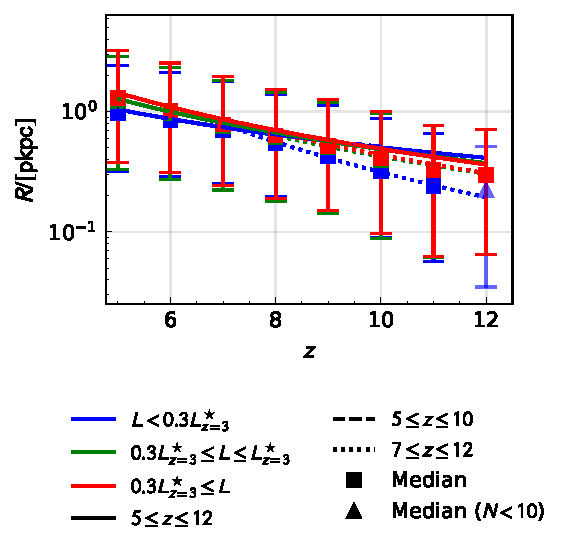
\includegraphics[width=\columnwidth]{Figures/Violin_ObsCompHalfLightRadius_evolution_pix_FAKE.TH.FUV_sim_default_All.pdf}
    \caption{The redshift evolution of galaxy size in the \flares\ sample split into 3 luminosity samples used in the literature: a low luminosity sample, $L < 0.3 \, L_{z=3}^{\star}$ (blue), an intermediate luminosity sample, $0.3 \, L_{z=3}^{\star} < L < L_{z=3}^{\star}$ (green), and a bright galaxy sample, $0.3 \, L_{z=3}^{\star}<L$ (red), where $L_{z=3}^{\star}\approx10^{29}$ erg s$^{-1}$ Hz$^{-1}$. We present 3 different fits the different redshift regimes: a solid line fit to the entire redshift range ($5 \leq z \leq 12$), a dashed line fit to a low-$z$ sample ($5 \leq z \leq 10$) and a dotted line fit to a high redshift sample ($7 \leq z \leq 12$). The low-$z$ fits and the full redshift range fits almost entirely overlap.
    The points show the median in each redshift bin with errorbars denoting the 16th and 84th percentile, a square point denotes more than 10 galaxies in the bin while a triangle denotes less than 10 galaxies present in the sample at that redshift.}
    \label{fig:evo}
\end{figure}

\begin{figure}
    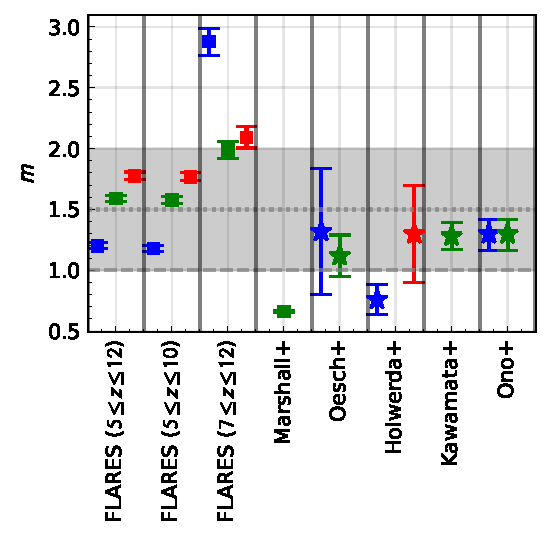
\includegraphics[width=\columnwidth]{Figures/SlopeComp_HalfLightRadius_evolution_pix_FAKE.TH.FUV_sim_default_All.pdf}
    \caption{A comparison to the slopes of the redshift size evolution derived from observations \citep{Oesch_2010, Ono_2013, Holwerda_2015, Kawamata_2018}, and the \bluetides\ simulation \citep{Marshall21}. Observations are denoted by stars and simulations are denoted by squares. The shaded range shows the range of slopes found in the FIRE-2 simulations \citep{Ma_18_size} for various fixed mass and luminosity galaxy samples. The dashed line corresponds to $m=1$, the theoretical scaling for systems of fixed mass \citep[e.g.][]{Bouwens_2004}, and the dotted line corresponds to $m=1.5$, the theoretical scaling for systems with fixed circular velocity \citep[e.g.][]{Ferguson_2004, Hathi_2008}. As with \fig{evo}, blue points represent a low luminosity sample ($L < 0.3 \, L_{z=3}^{\star}$), green points represent an intermediate luminosity sample ($0.3 \, L_{z=3}^{\star} < L < L_{z=3}^{\star}$), and red points represent a bright galaxy sample ($0.3 \, L_{z=3}^{\star}<L$).}
    \label{fig:evoslopes}
\end{figure}

In the literature there has been a wide range of presented methods for measuring the redshift evolution of galaxy sizes, with various approaches and galaxy sample definitions used for the computation. To produce a comprehensive comparison with \flares\ we employ non-linear least squares fitting (again using \texttt{scipy.curve\_fit}) to produce fits to \eq{evo} from various sample definitions pulled from the complete galaxy sample, all weighted with the \flares\ weighting scheme. The results of this fitting are presented in \tab{evo}.

In \fig{evo} we present these fits for a number of different sample definitions found in the literature. \fig{evoslopes} shows a comparison of the slope ($m$) from various studies, left to right: \flares, \cite{Marshall21}, \cite{Oesch_2010}, \cite{Holwerda_2015}, \cite{Kawamata_2018}, and \cite{Ono_2013}, with a shaded region representing the range of slopes from \cite{Ma_18_size}. We present the fitting parameters for these fits in \tab{evo}.

For the low luminosity sample we see a good agreement in slope between \flares\ and \cite{Oesch_2010} and \cite{Ono_2013}. For the other \flares\ samples we find comparatively high slopes compared to the other works. However, these values are in agreement with \cite{Ma_18_size} who predict values in the range $m=1-2$ depending on the fixed mass or luminosity regime (shown by the shaded region). All but the low luminosity sample's slopes are larger than the evolution of systems at fixed circular velocity, implying an increasing feedback contribution to the evolution with decreasing redshift. Conversely, the low luminosity sample's evolution is closer to that of a system at fixed mass with the same additional feedback contribution. As feedback becomes more efficient with decreasing redshift the star forming gas will be given more thermal energy and thus change the dynamics of the star forming gas, increasing the radii at which stars can form and thus the half light radii.

% The strongest tension exists between the \bluetides\ and \flares\ measurements. One possible suggestion for this discrepancy, as discussed in \cite{Marshall21}, is the limitation of \bluetides\ to galaxies at $z\geq7$, however when limiting the \flares\ sample to the redshifts in common between the two simulations the corresponding redshift slope instead increases to $m>2$ for all 3 samples. This leaves the aforementioned differences in the subgrid models, photometry modelling, and possibly more fundamentally the structure extraction method. Due to \bluetides's volume, running a halo finder was not feasible; instead, galaxies were extracted centred on black holes and associating particles inside the radius encompassing 200 times the critical stellar mass density (the critical density of the Universe multiplied by the baryon fraction and star formation efficiency of the simulation) of the black hole to that group, see \cite{Marshall21} for more details. This extraction method could bias galaxies towards slower evolution by including more unassociated stellar material at large radii as the IGM grows with redshift, leading to a suppression in the perceived size evolution. 

Limiting the included redshifts in the \flares\ sample can not only be used to compare to the more limited samples of \bluetides, with no galaxies at $z<7$, and observations, where $z\geq10$ galaxies are exceedingly rare, but can also probe the evolution of size during particular epochs. To do this we limited the sample to a high-$z$ sample limited to $z\geq7$ and a low-$z$ sample with $z\leq10$, the results of which are also included in \tab{evo}. Limiting to $z\geq7$ resulted in a large increase in the slope of the redshift evolution alongside unrealistically high normalisations, predicting $z=0$ sizes of the order $\sim300$ pkpc for the low luminosity sample and over double the $z=0$ size in the limited and high luminosity samples in the other redshift selections. Conversely, limiting to $z\leq10$ instead results in fitting results consistent with those produced by the full redshift range. This casts doubt on the sparse $z>10$ measurements in observations causing the differences in slope between the \flares\ measurement and observational measurements. More interestingly the differences in fits between redshift regimes implies a significantly faster evolution of galaxy size at the earliest times, even for the most dim and diffuse galaxies in the low luminosity sample. It is clear from \fig{evo} that a piecewise fit produces a considerably better fit to the data than fitting across the entire redshift range. 
% If \flares\ were extended beyond $z=5$ to lower redshift this could significantly affect the results presented here with this implied non-constant size evolution.

Tensions between \flares\ and the observations are far less stark than those between \flares\ and \bluetides\ samples but are nonetheless evident for the capped and high luminosity samples, we do however see a good agreement in the low luminosity sample. The tensions here could be explained by how sparse observations are at the highest redshifts due to the small area covered at the required depth; given that the low luminosity sample in \flares\ is also sparse at the highest redshifts, the agreement between observations and \flares\ here could be due to this luminosity regime being where the simulation and observations have the largest overlap in sampling strength. Additional observations from upcoming observatories populating the highest redshifts will increase the area and depth sampled in at this epoch and could rectify this tension. It should also be noted however that subgrid models require intensive investigation at this epoch, with comparison to robust observations to ascertain the validity of their behaviour. Future work will be able to converge the results of both simulations and observations to a consistent story of galaxy size evolution. 


\begin{table*}
\begin{center}
\begin{tabular}{ c | c | c | c | c | c | c | c }
 \hline
   & \multicolumn{2}{|c|}{$5 \leq z \leq 12$} & \multicolumn{2}{|c|}{$5 \leq z \leq 10$} & \multicolumn{2}{|c|}{$7 \leq z \leq 12$} \\ \hline
 Sample & $R_{0,z=0}/ [\mathrm{pkpc}]$ & $m$ & $R_{0,z=0}/ [\mathrm{pkpc}]$ & $m$ &  $R_{0,z=0}/ [\mathrm{pkpc}]$ & $m$ \\ \hline
 $L<0.3L_{z=3}^{\star}$ 
 & 8.99$\pm$0.42  & 1.20$\pm$0.03
 & 8.65$\pm$0.41  & 1.18$\pm$0.03
 & 311.78$\pm$73.80 & 2.88$\pm$0.11\\  
 $0.3L_{z=3}^{\star}<L<L_{z=3}^{\star}$ 
 & 21.98$\pm$1.04  & 1.59$\pm$0.03
 & 21.53$\pm$1.04   & 1.58$\pm$0.03
 & 49.91$\pm$7.62  & 1.99$\pm$0.07 \\ 
 $0.3L_{z=3}^{\star}<L$ 
 & 34.61$\pm$2.08  & 1.78$\pm$0.03
 & 34.11$\pm$2.09  & 1.77$\pm$0.03
 & 66.22$\pm$12.43  & 2.09$\pm$0.09\\ 
 \hline
\end{tabular}
\caption{The fitting parameters for \eq{evo} in \fig{evo} split into 3 redshift samples. From left to right: the full \flares\ sample, a sample excluding the highest redshifts where robust observations are sparse, and a sample excluding the lowest redshift snapshots for comparison to \bluetides. $R_{0,z=0}$ is a normalisation factor corresponding to a galaxy's size at $z=0$ and $m$ is the slope of the redshift evolution.}
\label{tab:evo}
\end{center}
\end{table*}

